% ==============================================================================
%                                    DVG303
%                  Objektorienterad design och programmering
%                                Laboration #1
%
% Author:   Jonas Sjöberg
%           Högskolan i Gävle
%           tel12jsg@student.hig.se
%           https://github.com/jonasjberg
%
% License:  Creative Commons Attribution-NonCommercial-ShareAlike 4.0
%           International.  See LICENSE.md for full licensing information.
% ==============================================================================

\renewcommand{\thesubsection}{(\alph{subsection})}

\section{Uppgift 1}\label{sec:uppg1}
% \addcontentsline{toc}{section}{Uppgift 1}


\subsection{}\label{sec:uppg1a}
\subsubsection*{Frågeställning}
Modellera klasserna som representerar konkreta geometriska figurer som ska
kunna hanteras i programmet och därför ska ingå i programmets datamodell:
Punkt, linje, triangel, cirkel, rektangel.
\par Beskriv klasserna på ett liknande sätt som i kursboken, kap 2.2, på sida
65 - tredje upplaga.  Skapa dessutom ett UML-klassdiagram för modellen.
\par Motivera era beslut: Varför skapade ni modellen som den är? Varför har
klasserna de attribut och operationer så som ni valde?

\subsubsection*{Lösning}
Figurerna beskrivs av ett visst antal punkter eller positioner som
representeras av \texttt{Vertex2D}-instanser. Alla figurer består av minst ett
\texttt{Vertex2D}-objekt som representerar figurens mittpunkt. Figurerna kan
delas upp i två separata grenar i arvshierarkin, \texttt{Figure} och
\texttt{SimpleFigure}.  Skillnaden mellan Figure och SimpleFigure är hur många
punkter de lagrar för att beskriva figuren de representerar.  Figurer som kan
beskrivas med bara en \texttt{Vertex2D}-instans, figurens position, ärver från
\texttt{SimpleFigure}; punkt, cirkel och ellips.  Figurer som består av fler
\texttt{Vertex2D}-objekt, ärver från \texttt{Figure}.  Klassen \texttt{Figure}
lagrar sina punkter i en lista för enkel åtkomst.  Det möjliggör också
skapandet av figurer med ett godtyckligt antal punkter.

\begin{figure}[htbp]
\centering
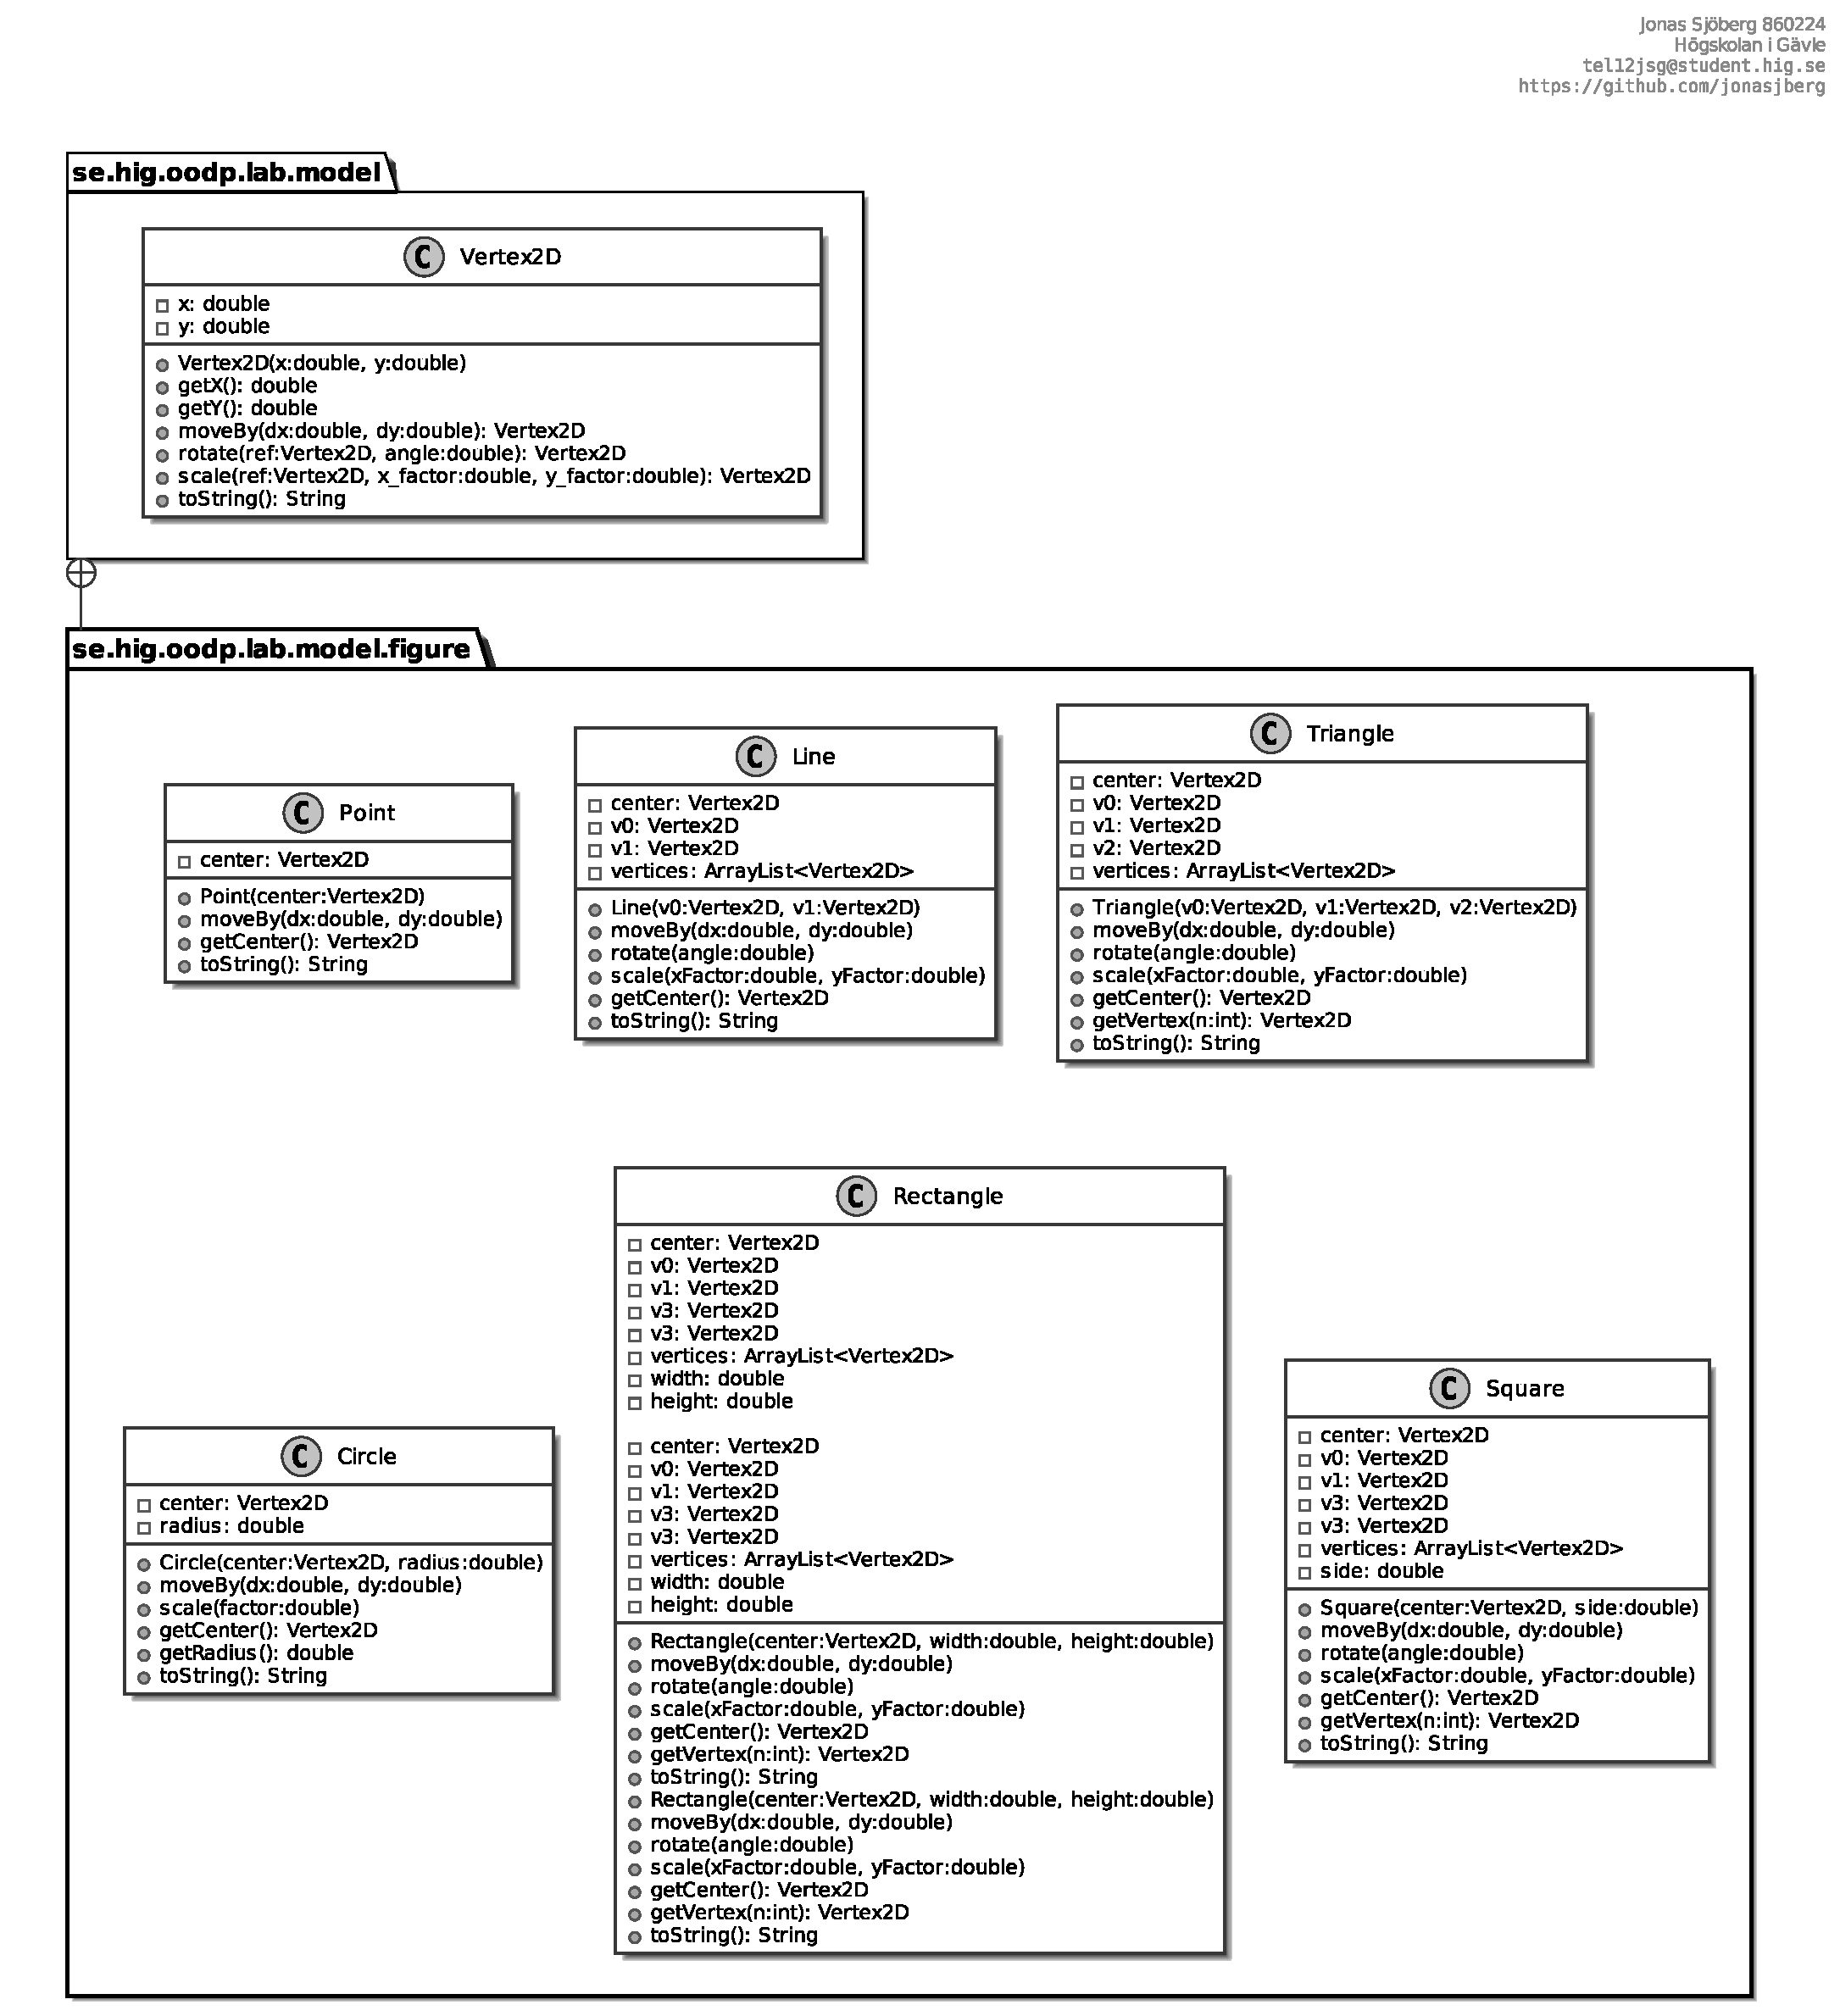
\includegraphics[width=\linewidth]{diagram/uppgift1.eps}
\caption{Uppgift~1\ref{sec:uppg1a}: UML-diagram för geometriska figurer
(\texttt{diagram/uppgift1.eps})}
\label{fig:uppg1a}
\end{figure}

\par UML-klassdiagrammet återfinns i Figur~\ref{fig:uppg1a}, samt bifogad fil.


\subsection{}\label{sec:uppg1b}
\subsubsection*{Frågeställning}
Implementera klasserna som ingår i klassdiagrammet och skapa JUnit-tests för
att testa koden!

\subsubsection*{Lösning}
Se bifogad källkod, klasserna finns i paketen
\texttt{se.hig.oodp.lab.model.simplefigure} \\ och
\texttt{se.hig.oodp.lab.model.figure}.



\subsection{}\label{sec:uppg1c}
\subsubsection*{Frågeställning}
Vilken relation ser ni mellan klassen Vertex2D och figurklasserna resp. mellan
instanser av Vertex2D och instanser av figurklasserna? På vilket sätt
återspeglas relationen i klassdiagrammet? Ge en förklaring!

\subsubsection*{Lösning}
Klassen \texttt{Vertex2D} är en del av figurklasserna. Figurklasserna består
av minst en \texttt{Vertex2D} som utgör figurens mittpunkt. Figurklasserna
har en varsin lista där ett godtyckligt antal \texttt{Vertex2D}-objekt kan
lagras, antalet beror på vilken figur subklassen representerar.
